% http://www.LaTeXTemplates.com
\documentclass[a0paper,portrait]{baposter}

\usepackage[font=small,labelfont=bf]{caption} % Required for specifying captions to tables and figures
\usepackage{booktabs} % Horizontal rules in tables
\usepackage{relsize} % Used for making text smaller in some places
\usepackage{amsmath}
\usepackage{fixltx2e}
\usepackage{caption}
\usepackage{mathtools}
\usepackage{graphicx}


\graphicspath{{fig/}} % Directory in which figures are stored

\definecolor{bordercol}{RGB}{244, 89, 66} % Border color of content boxes
\definecolor{headercol1}{RGB}{244, 89, 66} % Background color for the header in the content boxes (left side)
\definecolor{headercol2}{RGB}{244, 244, 65} % Background color for the header in the content boxes (right side)
\definecolor{headerfontcol}{RGB}{0,0,0} % Text color for the header text in the content boxes
\definecolor{boxcolor}{RGB}{237, 255, 250} % Background color for the content in the content boxes 186,215,230

\begin{document}

\background{ % Set the background to an image (background.pdf)
\begin{tikzpicture}[remember picture,overlay]
\draw (current page.north west)+(-2em,2em) node[anchor=north west]
{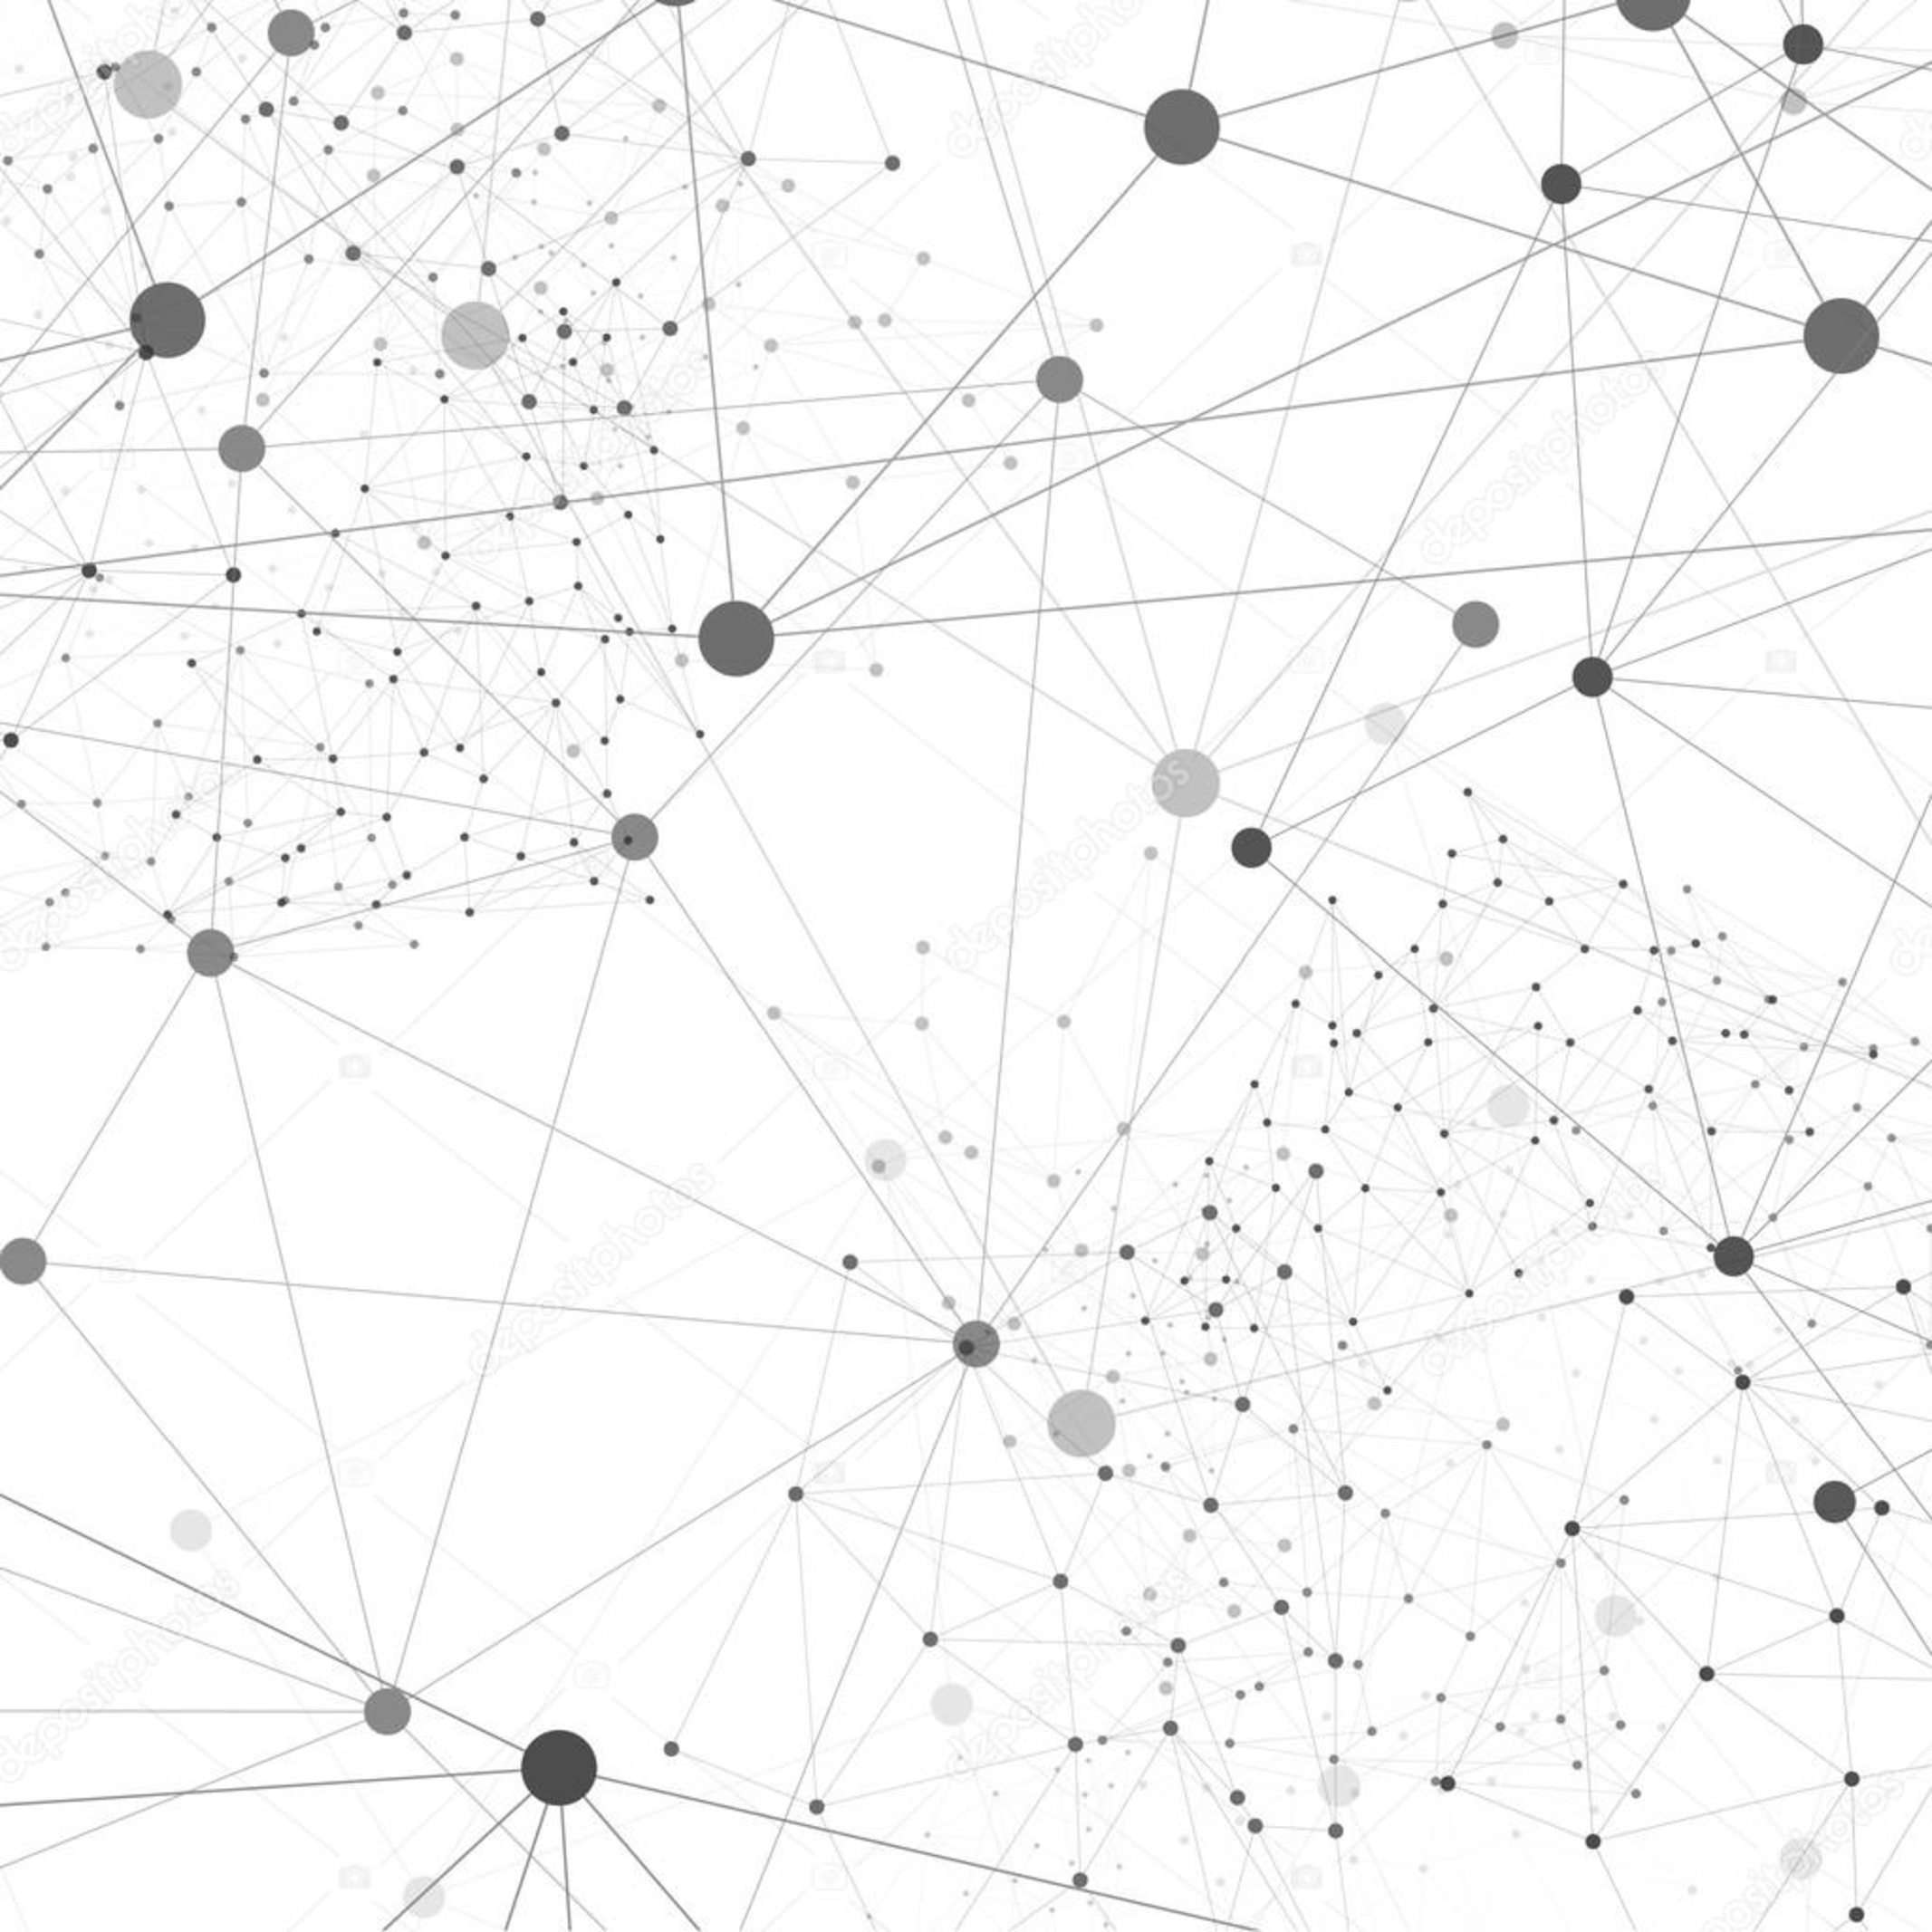
\includegraphics[height=1.1\textheight]{background}};
\end{tikzpicture}
}

\begin{poster}{
grid=false,
borderColor=bordercol, % Border color of content boxes
headerColorOne=headercol1, % Background color for the header in the content boxes (left side)
headerColorTwo=headercol2, % Background color for the header in the content boxes (right side)
headerFontColor=headerfontcol, % Text color for the header text in the content boxes
boxColorOne=boxcolor, % Background color for the content in the content boxes
headershape=roundedright, % Specify the rounded corner in the content box headers
headerfont=\Large\sf\bf, % Font modifiers for the text in the content box headers
textborder=rectangle,
background=user,
headerborder=open, % Change to closed for a line under the content box headers
boxshade=plain
}
{}
%
%----------------------------------------------------------------------------------------
%	TITLE AND AUTHOR NAME
%----------------------------------------------------------------------------------------
%
{\sf\bf Synchronization of Type 1 Phase Oscillators on Directed Acyclic Graphs} % title
{\vspace{-0.2em} \smaller \textbf{\textcolor{red}{Abolfazl Ziaeemehr}}\textsuperscript{1}, 
	\textbf{\textcolor{red}{Mina Zarei}}\textsuperscript{1,2}\\ % Author names
{\smaller 1. Institute for Advanced Studies in Basic Sciences (IASBS), Zanjan, Iran} \\
{\smaller 2. School of Computer Science, Institute for Research in Fundamental Sciences (IPM), Tehran, Iran.}
} % Author email addresses
{
\includegraphics[scale=0.25]{logo}} % University/lab logo

%----------------------------------------------------------------------------------------
%	INTRODUCTION
%----------------------------------------------------------------------------------------

\headerbox{Abstract}{name=introduction,column=0,row=0}{
We study the effects of directionality on synchronization of dynamical networks. Performing the linear stability analysis and the numerical simulation of the Kuramoto model in directed networks, we show that balancing in- and out-degrees of all nodes enhances the synchronization of sparse networks, especially in networks with high clustering coefficient and homogeneous degree distribution.
Furthermore, by omitting all the feedback loops, we show that while hierarchical directed acyclic graphs are structurally highly synchronizable, their global synchronization is too sensitive to the choice of natural frequencies and is strongly affected by noise.
}

%----------------------------------------------------------------------------------------
%	MATERIALS AND METHODS
%----------------------------------------------------------------------------------------

\headerbox{Methods}{name=methods,column=0,below=introduction}
{
The Kuramoto model~\cite{kuramoto2003chemical} consists of a collection of $N$ coupled phase oscillators, $\theta_i$, having natural frequencies $\omega_i$  distributed
with a given probability density and its time evolution is given by:
\begin{align*}
&\dot{\theta}_i=\omega_i+\frac{\kappa}{N} \sum_{j=1}^{N} a_{ij} \Big[ u\sin(\theta_j-\theta_i)\\
	&\hspace{1.15cm}+(1-u)\frac{(1-cos(\theta_j-\theta_i))}{2} \Big],
\end{align*}
%\begin{align*}
%&\dot{\theta}_i=\omega_i+\frac{\kappa}{N} \displaystyle {\sum_{j=1}^{N} a_{ij} G(\theta_i,\theta_j) ,}\\
%& G(\theta_i,\theta_j)= u\sin(\theta_j-\theta_i)+(1-u)\frac{(1-cos(\theta_j-\theta_i))}{2}
%\end{align*}
where $\kappa$ shows the overall coupling strength. 
To quantify the degree of synchrony, the phase order parameter is defined as $r(t)= {1\over N} {\langle | \sum_{i=1}^{N} \mathrm{e}^{i\theta_{i}(t)}| \rangle}$,  where $0\leq r\leq{1}$ measures the phase coherence of oscillators. The value $r=1$ shows the fully synchronized state, while $r=0$ indicates the incoherent solution. Here, $\langle\dots\rangle$ indicates averaging over different network realizations and initial conditions. The time average of $r$ after achieving a steady state is represented  by $R$. In our simulations, the initial values of $\theta_i$ are randomly drawn from a uniform distribution in interval $[0, 2\pi]$, and natural frequencies are identical.
}
%----------------------------------------------------------------------------------------
%	CONCLUSION
%----------------------------------------------------------------------------------------

\headerbox{Conclusion}{name=conclusion,column=0,below=methods}{
The purpose of this report is to investigate the effect of structure on synchronization of type I and II oscillators~\cite{ermentrout1996type,Mofakham2018} and to find an optimum structure for type I oscillators to synchronize.  We show that feed forward loops help the synchrony of homogeneous type I oscillators. This is also true for networks with hubs (Scale free networks). Actually the information flow start from hubs in these networks. 
}

%----------------------------------------------------------------------------------------
%	REFERENCES
%----------------------------------------------------------------------------------------

\headerbox{References}{name=references,column=0,below=conclusion, above=bottom}{

\smaller % Reduce the font size in this block
\renewcommand{\section}[2]{\vskip 0.05em} % Get rid of the default "References" section title
%\nocite{*} % Insert publications even if they are not cited in the poster

\bibliographystyle{unsrt}
\bibliography{lib} % Use sample.bib as the bibliography file
}

%----------------------------------------------------------------------------------------
%	ACKNOWLEDGEMENTS
%----------------------------------------------------------------------------------------

%\headerbox{Acknowledgements}{name=acknowledgements,column=0,below=references, above=bottom}{
%
%\smaller % Reduce the font size in this block
%Fusce mattis tellus ac odio imperdiet lobortis. Cum sociis natoque penatibus et magnis dis parturient montes, nascetur ridiculus mus. Phasellus commodo blandit euismod. Ut porttitor cursus magna. Mauris adipiscing pellentesque ipsum nec facilisis. Cras ornare bibendum bibendum. Ut a elit purus, vel adipiscing.
%} 

%----------------------------------------------------------------------------------------
%	RESULTS 1
%----------------------------------------------------------------------------------------

\headerbox{Lyapunov spectrum analysis on motifs and network properties}{name=results1,span=2,column=1,row=0}
{ % To reduce this block to 1 column width, remove 'span=2'
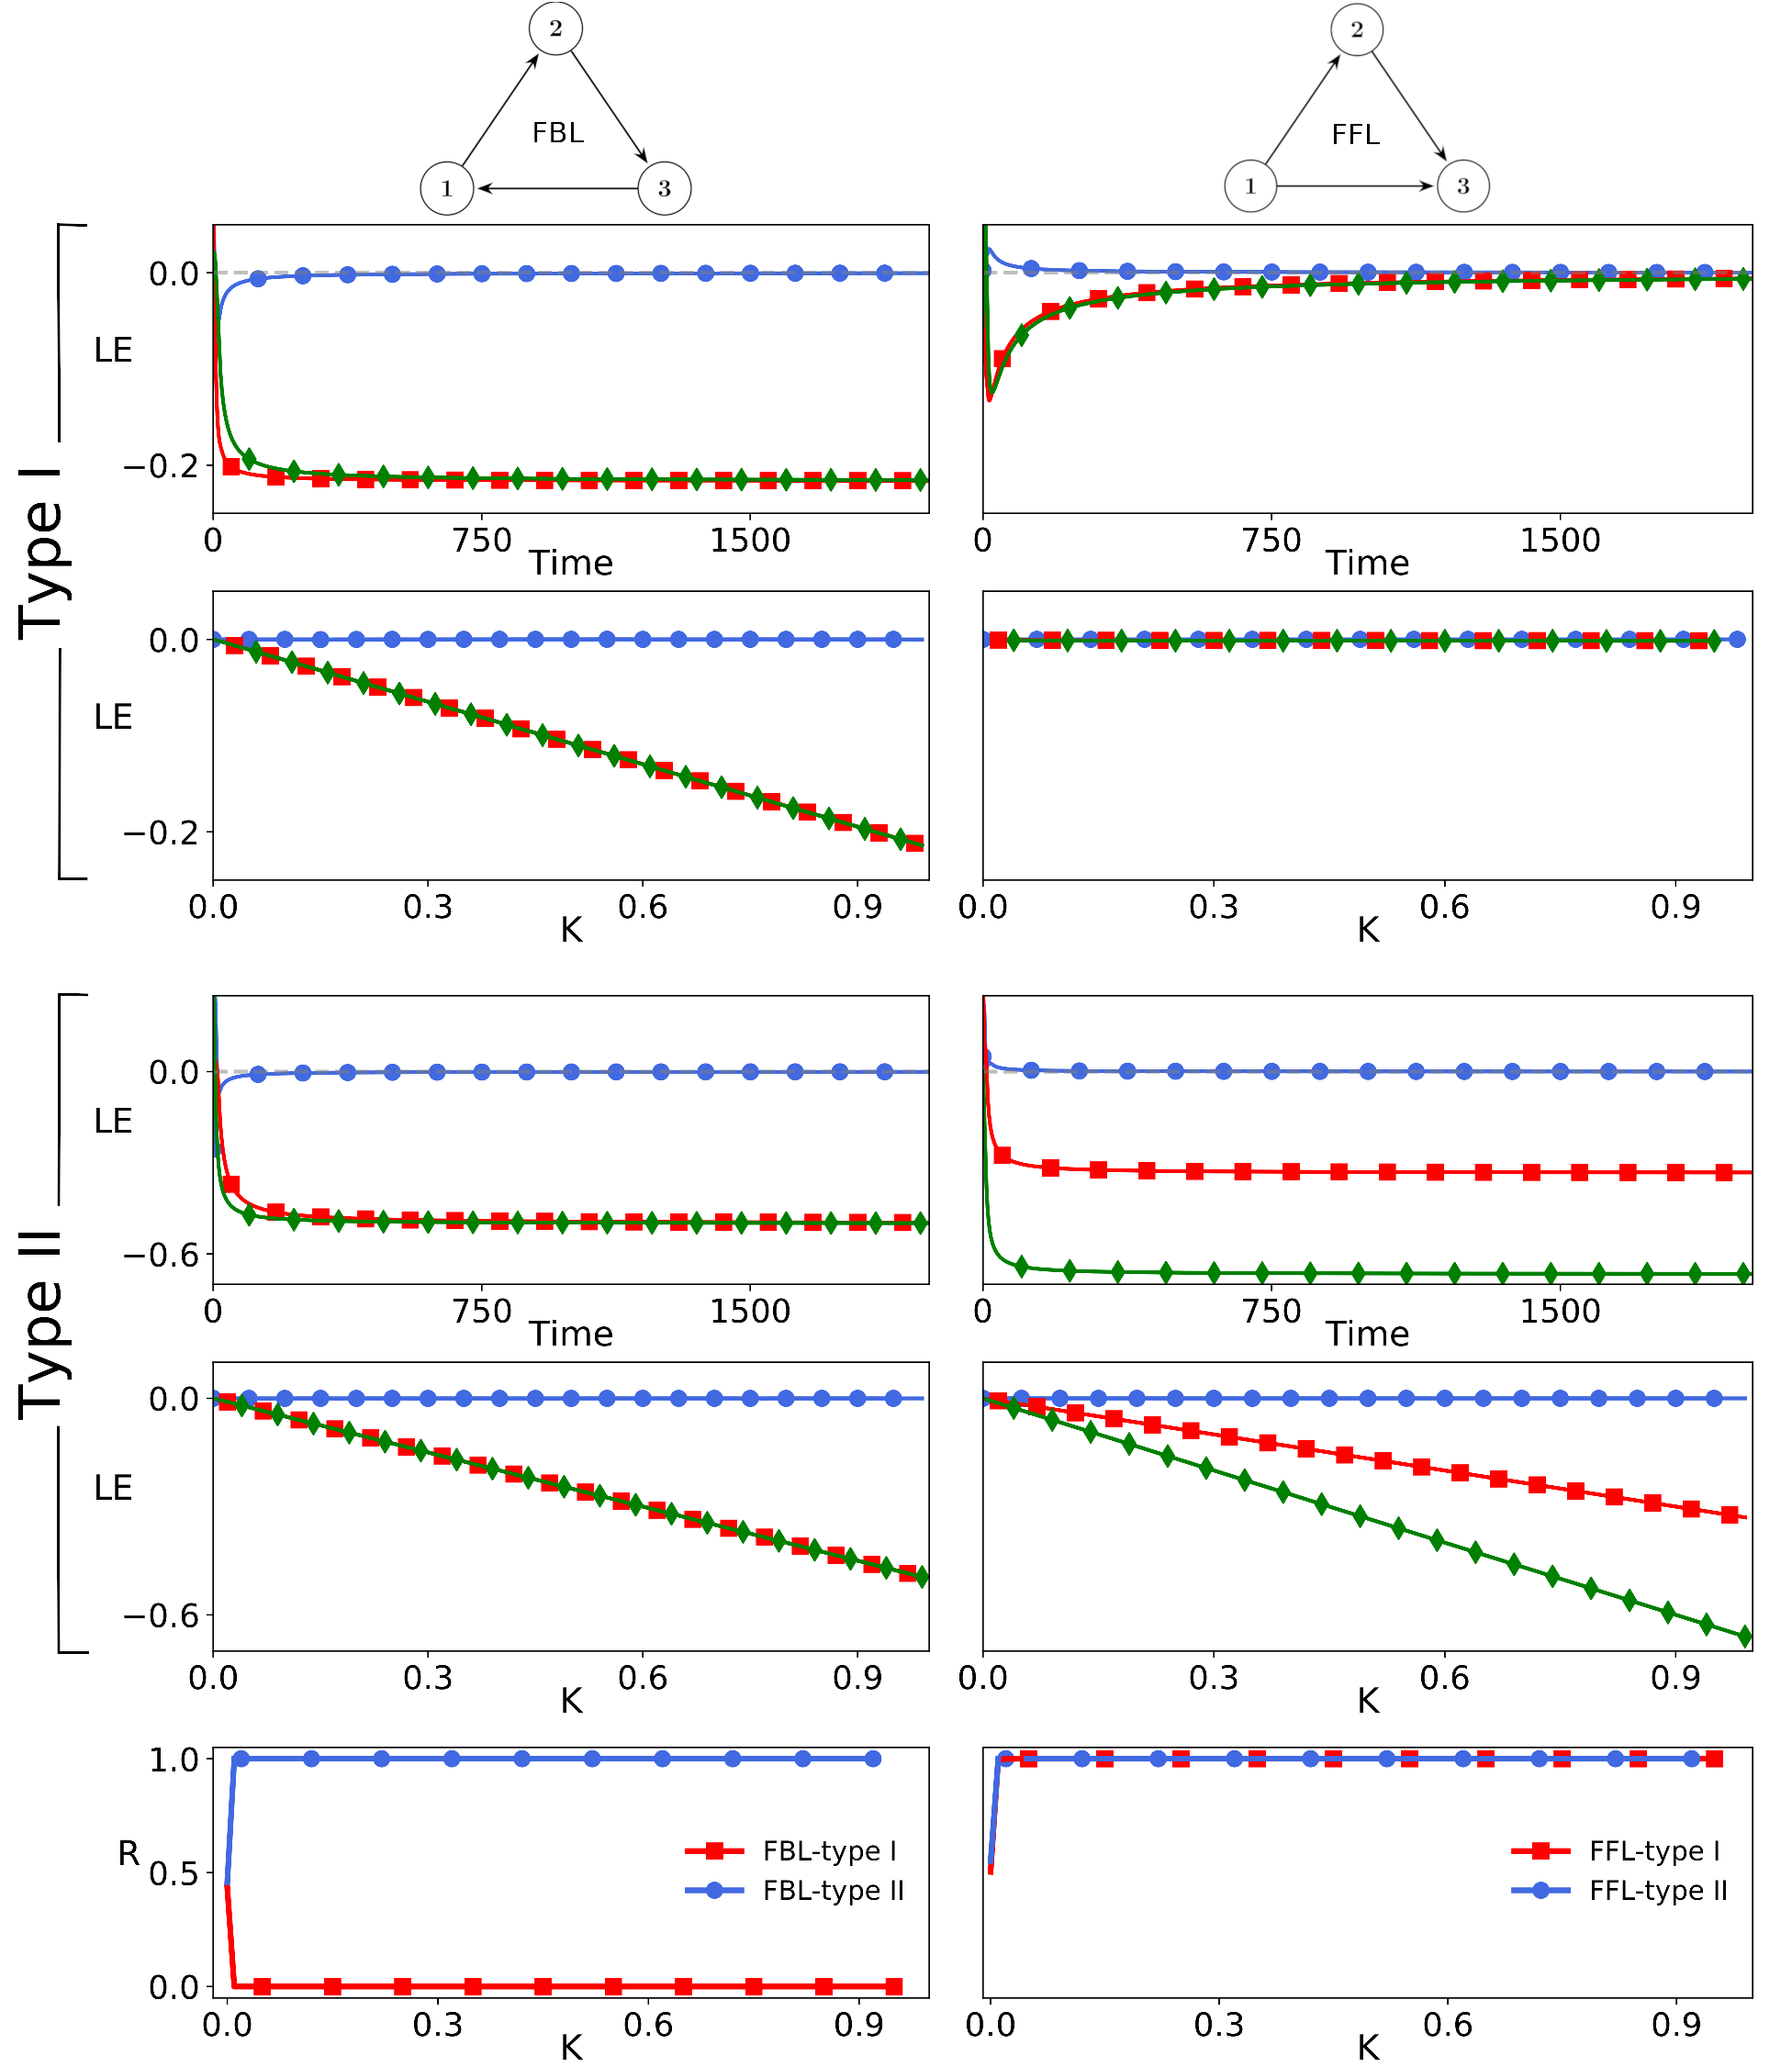
\includegraphics[scale=0.18]{fig/loops}
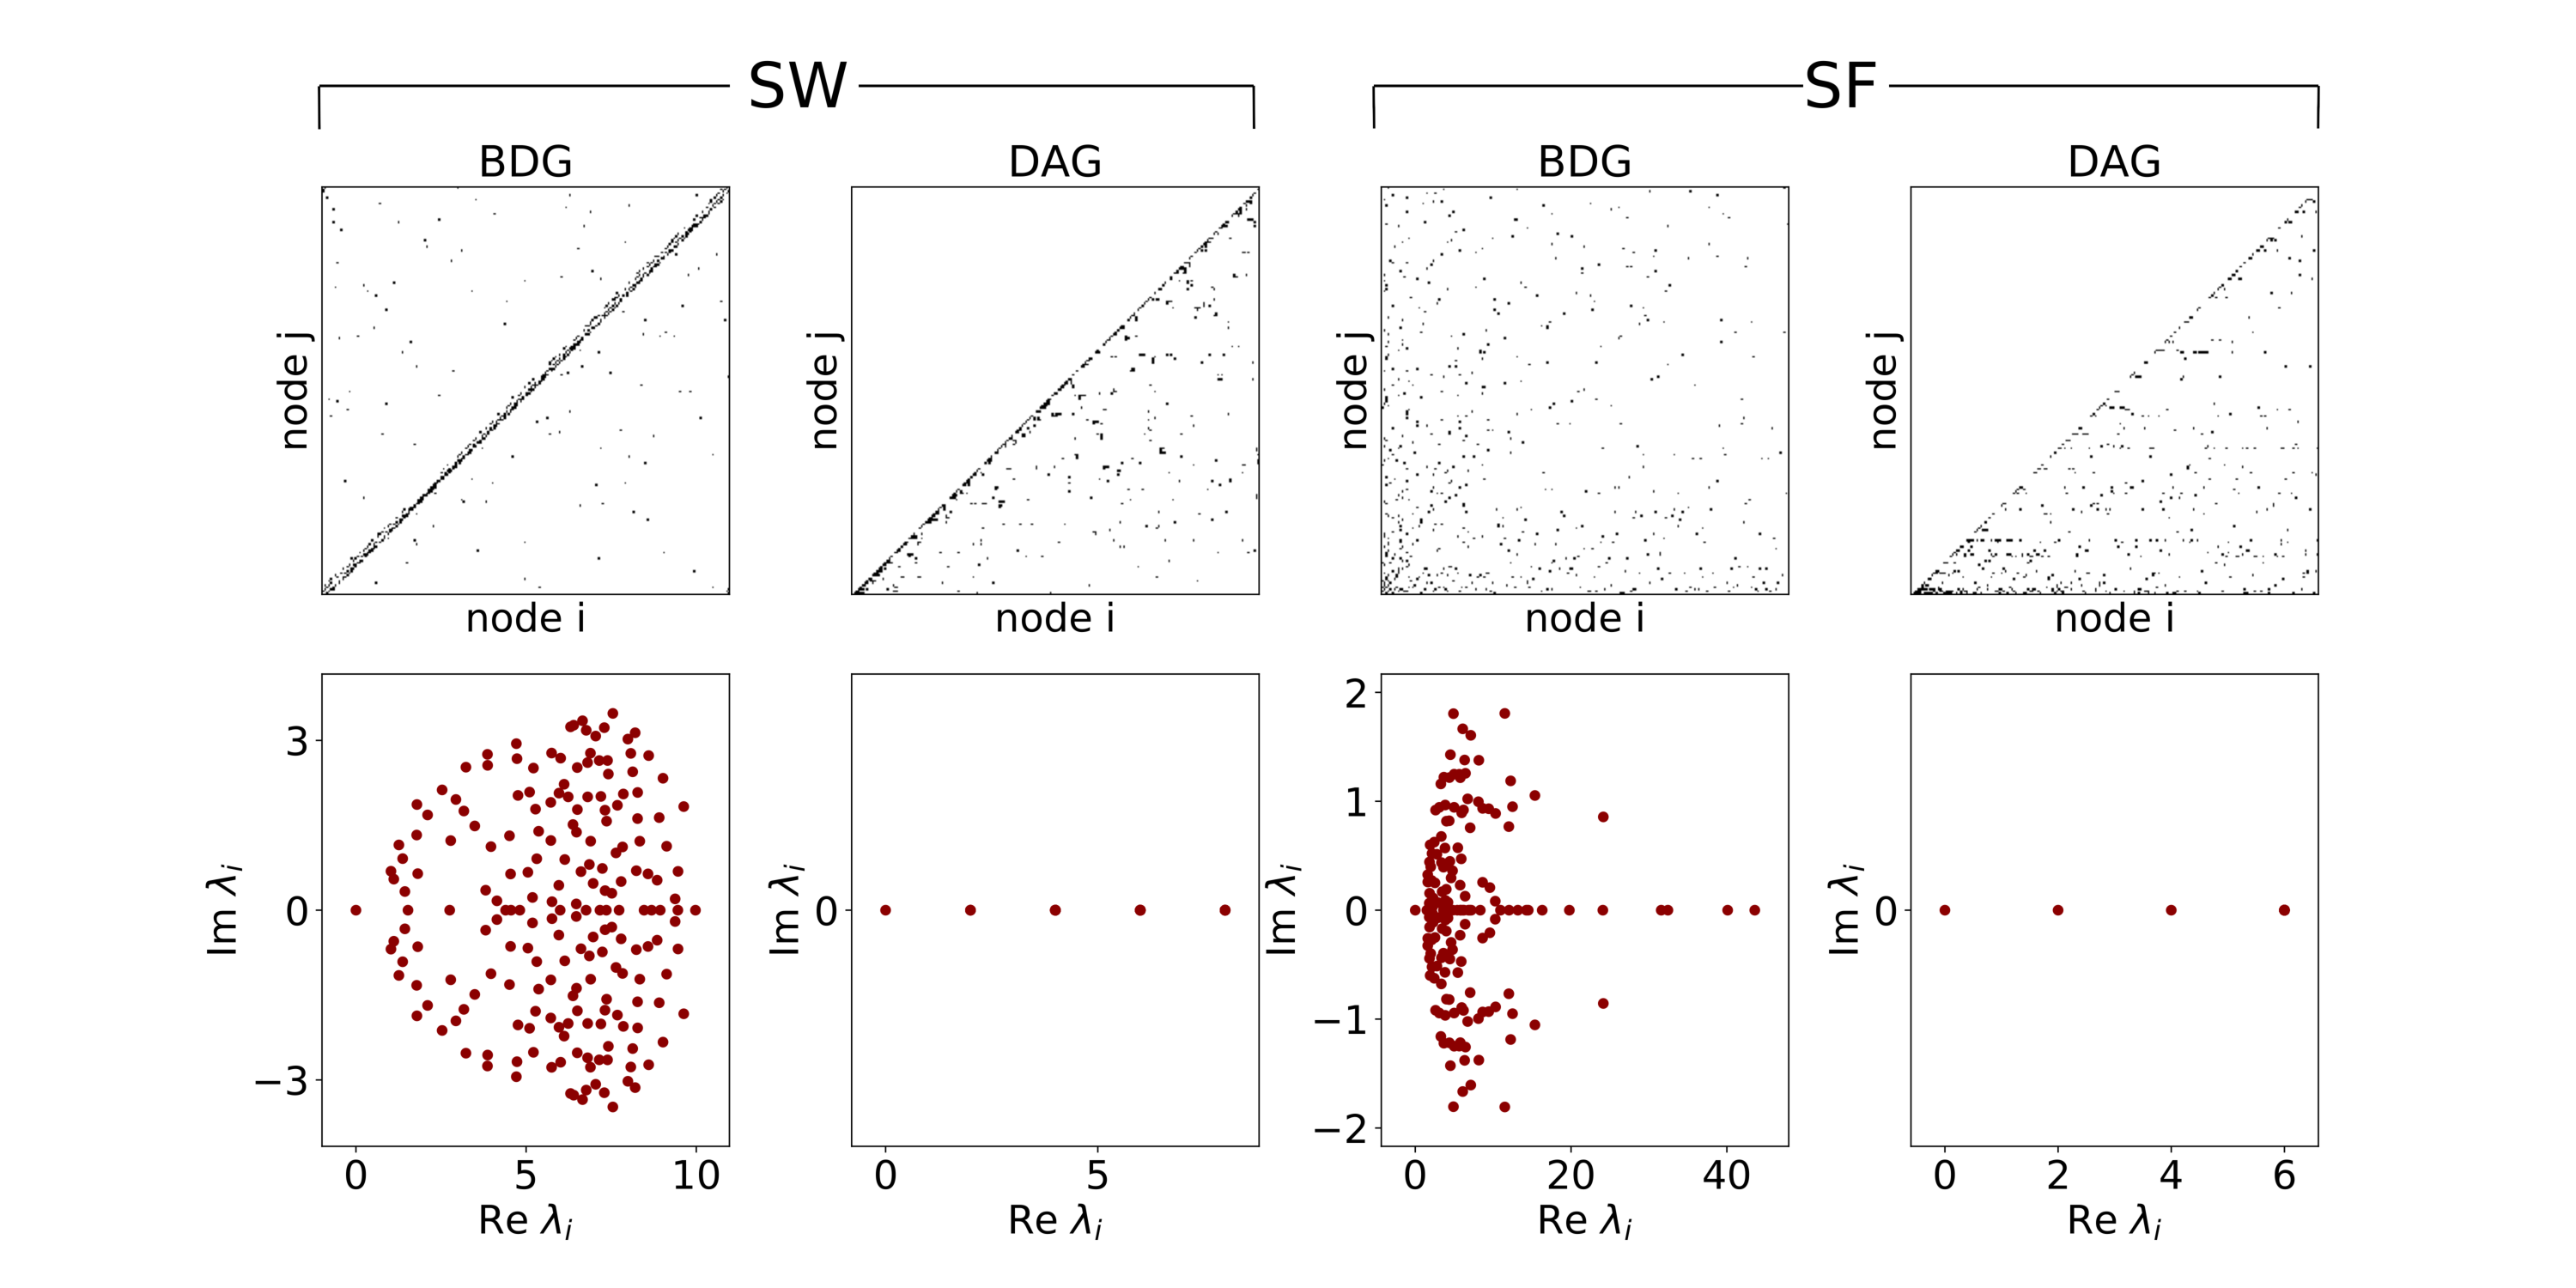
\includegraphics[scale=0.22, trim=4cm 0cm 4cm 1cm,clip]{directioning}

\captionof{figure}{
	\textbf{ (LEFT PANEL) Synchronization stability of FBL and FFL motifs.} Lyapunov exponents and order parameter versus time and coupling for identical type I or type II  phase ossillators connected by FBL (Left column) and FFl (right column) loops.\\
	\textbf{(RIGHT PANEL) Properties of two different directed networks. } Adjacency matrix (top) and Eigenvalues of the Laplacian
	matrix (bottom), for small world  and scale free Balanced Directed Graphs (BDGs) and Directed Acyclic Graphs(DAGs) with N=200 nodes.
	}
}

%----------------------------------------------------------------------------------------
%	RESULTS 2
%----------------------------------------------------------------------------------------
%{name=results2,span=2,column=1,below=results1,above=bottom}
\headerbox{Lyapunov spectrum analysis and synchronizations of networks}{name=results2,span=2,column=1,below=results1,above=bottom}{ % To reduce this block to 1 column width, remove 'span=2'
	\begin{center}
		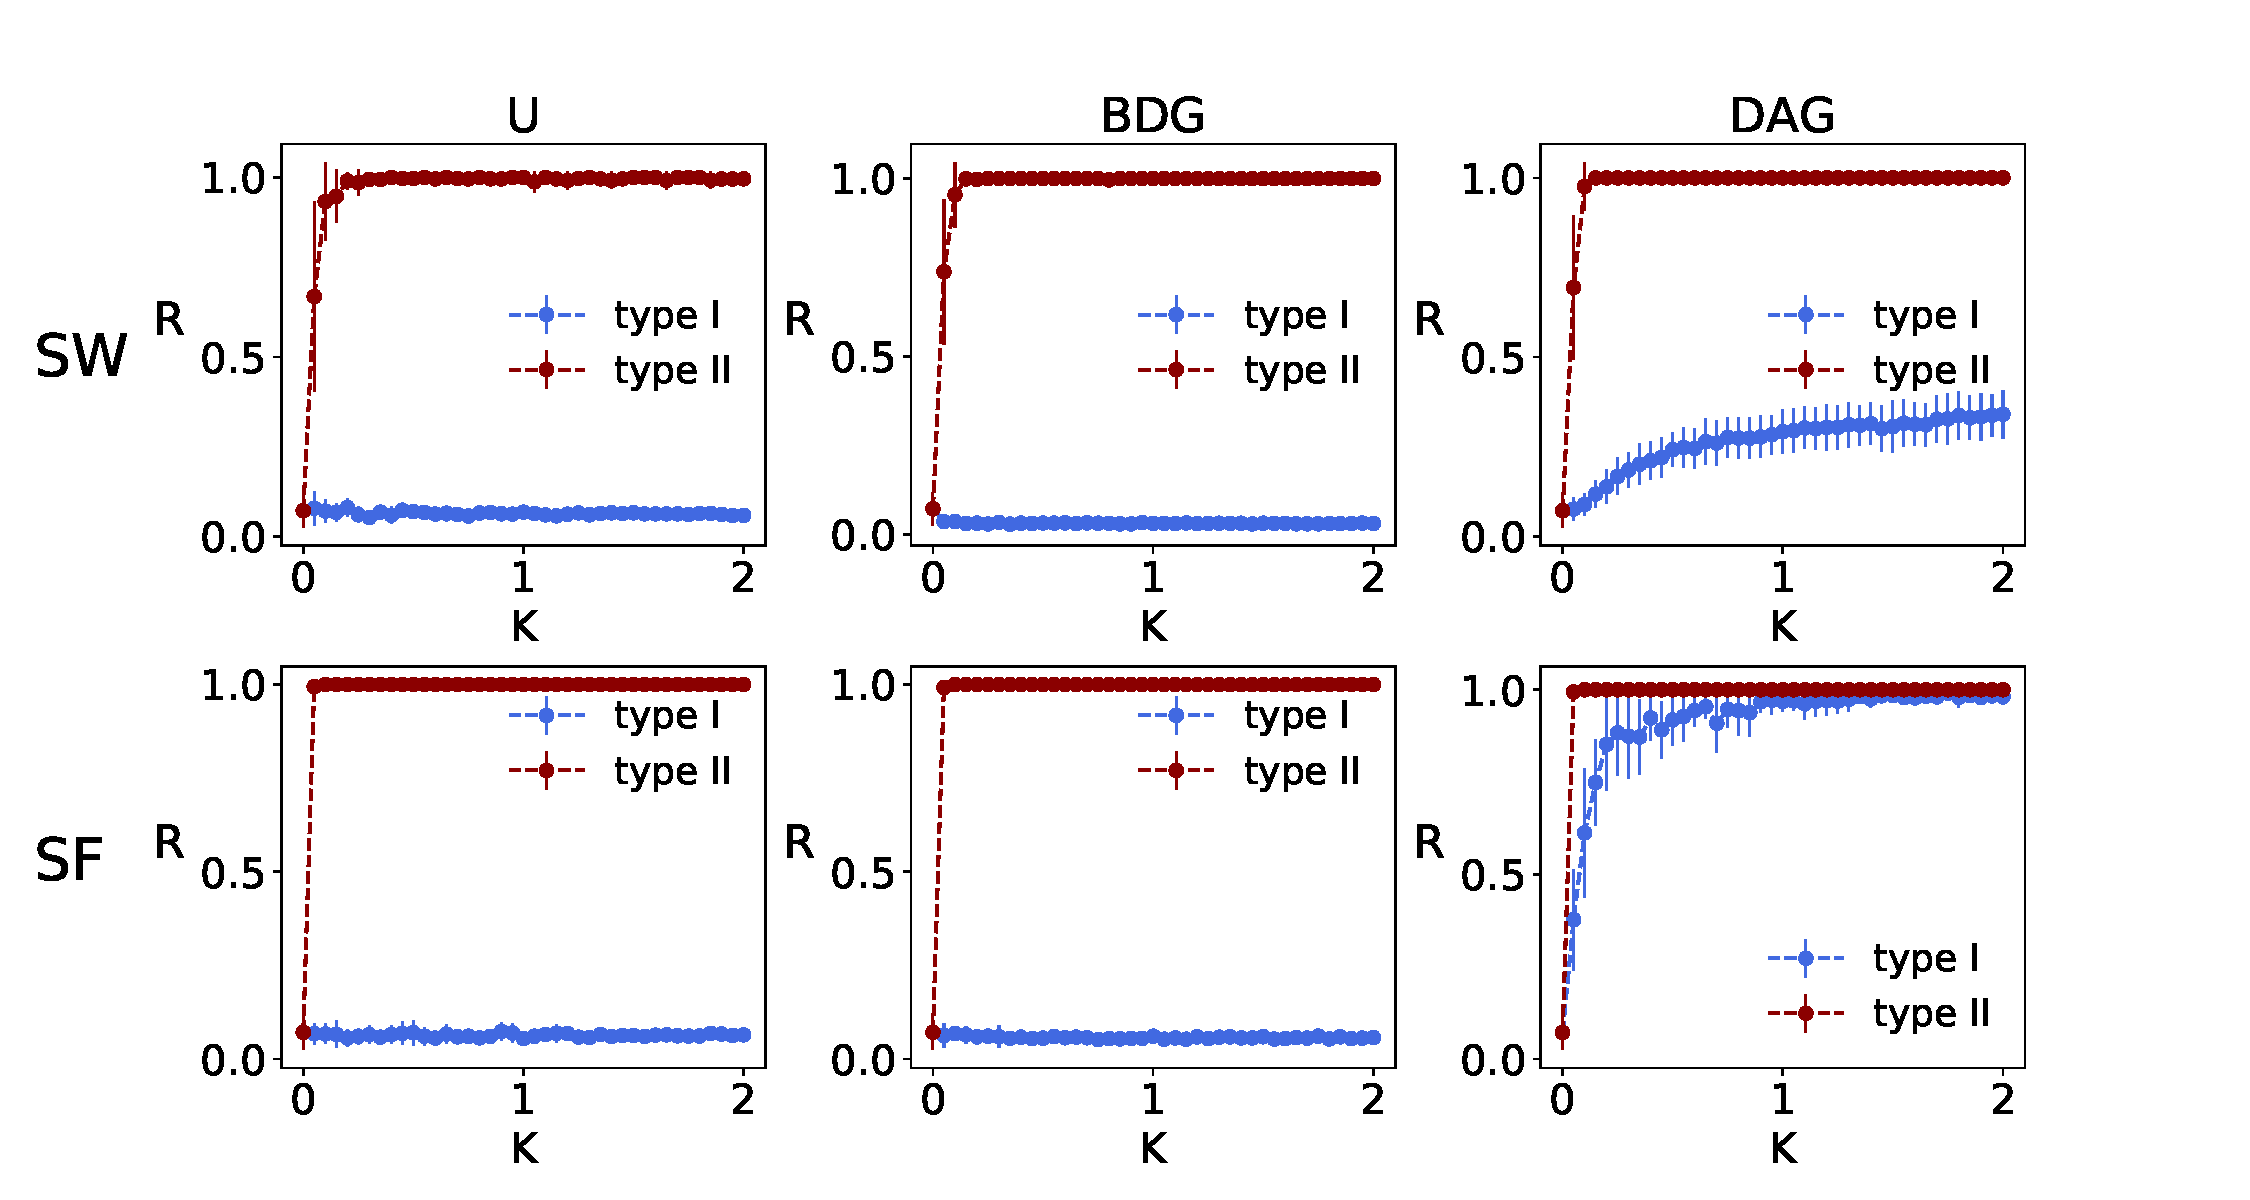
\includegraphics[scale=0.28, trim=0cm 0cm 3cm 1cm,clip]{fig/orderparameter}
		\captionof{figure}
		{
			\textbf{Comparison of phase synchronizability of identical type I and type II oscillators on different network structures. } Stationary order parameter  versus coupling strength  of the small-world (top) and scale-free (bottom) networks with  different link directionalities (U(Undirected), BDG(Balanced Directed graph) and DAG(directed Acyclic graph)). Here, $N=200$ and the results averaged over 30 network realizations and random initial phases.
		}
	\end{center}
	
	\begin{center}
		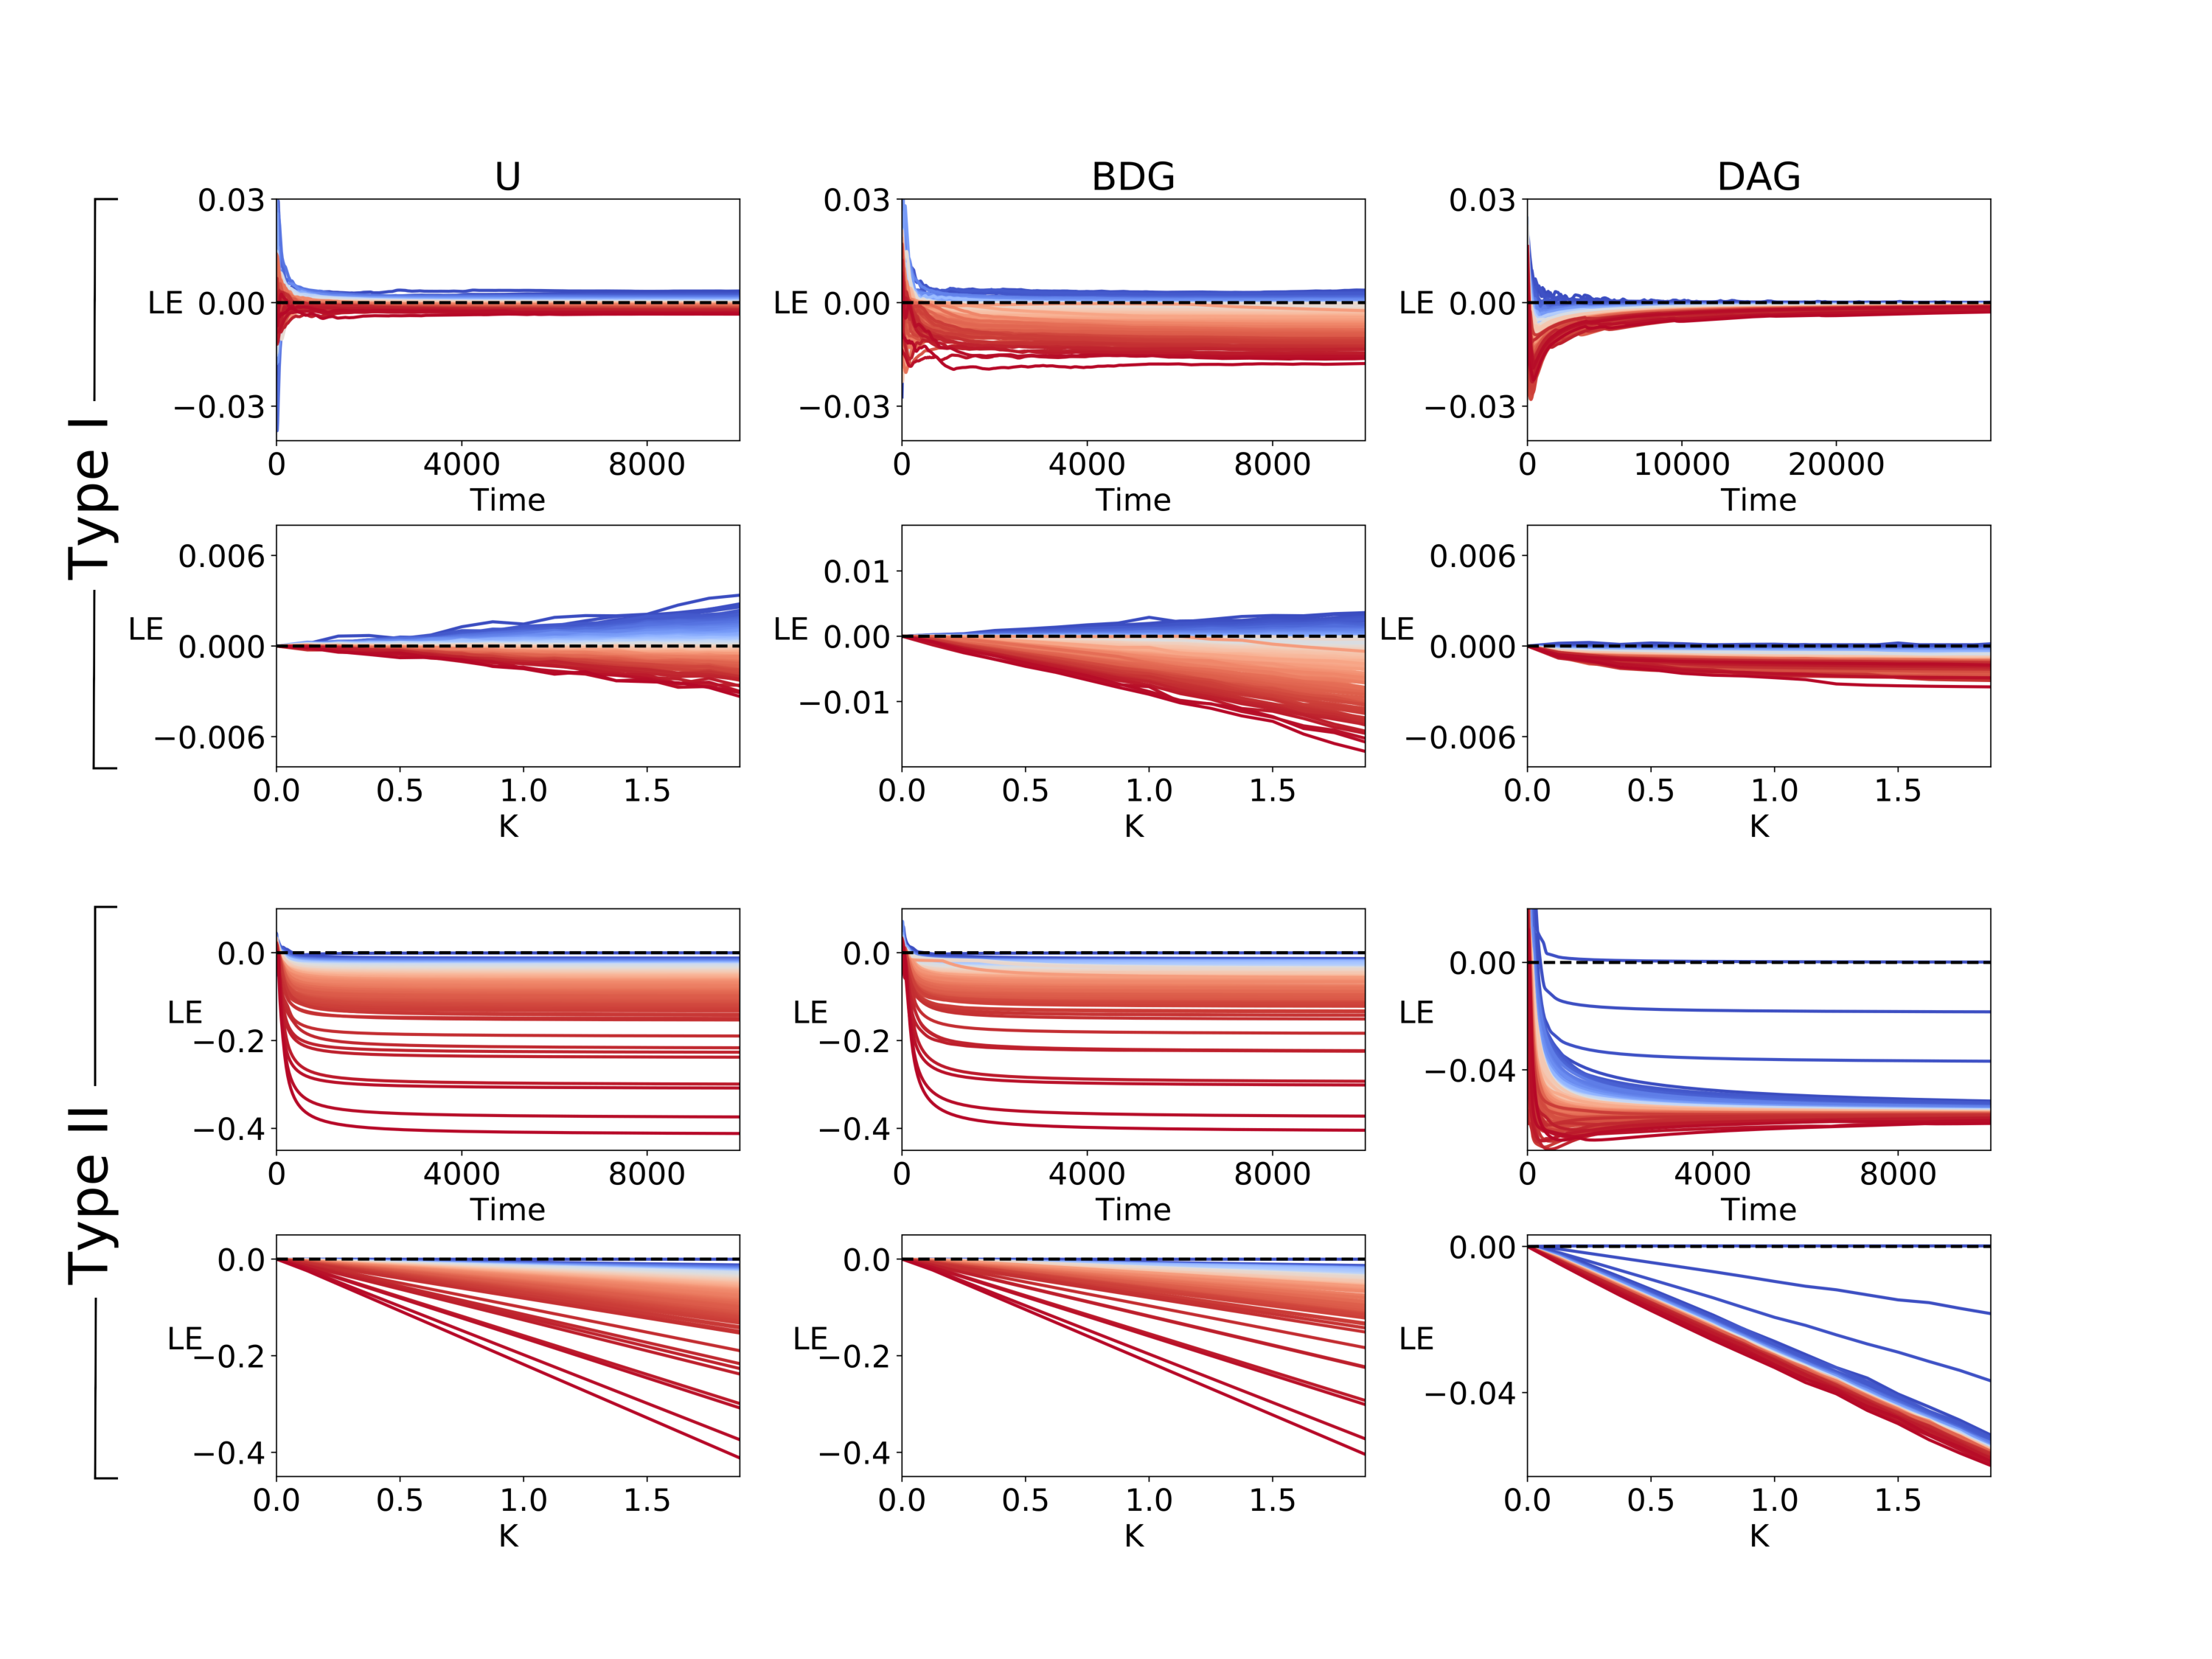
\includegraphics[scale=0.23, trim=1cm 1cm 4cm 3cm, clip]{fig/bdg-dag}
		\captionof{figure}{
			\textbf{ Comparison of synchronizability of identical type I and type II oscillators on scale-free networks with different directionalities based on Lyapunov exponents }. Lyapunov exponents versus time and coupling strength  for type I (top) or type II(bottom) phase oscillators situated on undirected graphs, BDGs and DAGs, with \textbf{N=200} nodes.}
	\end{center}


}

%----------------------------------------------------------------------------------------

\end{poster}

\end{document}